\subsection{Metric Tensor}

The length of a vector in an arbitrary coordinate system is defined by its norm which in
turn is defined by the scalar product:
\begin{equation}
    \begin{array}{rcl}
        \|\vec{v}\|^2 & = & \vec{v} \cdot \vec{v} \\
        \noalign{\vskip10pt}
        & = & (v^1 \hdbv{1} + v^2 \hdbv{2}) \cdot (v^1 \hdbv{1} + v^2 \hdbv{2}) \\ 
        & = & (v^1)^2(\hdbv{1}\cdot\hdbv{1}) + v^1 v^2 (\hdbv{1}\cdot\hdbv{2}) +
               v^2 v^1 (\hdbv{2}\cdot\hdbv{1}) +(v^2)^2(\hdbv{2}\cdot\hdbv{2}) \\
        & = & (v^1)^2(\hdbv{1}\cdot\hdbv{1}) + 2 v^1 v^2 (\hdbv{1}\cdot\hdbv{2}) +
              (v^2)^2(\hdbv{2}\cdot\hdbv{2}) \\
        \noalign{\vskip10pt}
        & = & (\tilde{v}^1)^2(\hdbtv{1}\cdot\hdbtv{1}) + 2 \tilde{v}^1 \tilde{v}^2 (\hdbtv{1}\cdot\hdbtv{2}) +
              (\tilde{v}^2)^2(\hdbtv{2}\cdot\hdbtv{2})              
    \end{array}
\end{equation}

In orthogonal coordinate systems the mixed products $(\hdbv{1}\cdot\hdbv{2})$ and
$(\hdbtv{1}\cdot\hdbtv{2})$ are equal to $0$, but in the more general non-orthogonal case
these terms do not disappear. \\

The scalar product can be written in component form based on the summation convention with
an implied summation over $i$ and $j$ as
\begin{equation}
    \begin{array}{rcl}
        \|\vec{v}\|^2 = \vec{v} \cdot \vec{v} & = & (v^i \hdbv{i}) \cdot (v^j \hdbv{j})
                        = v^i v^j (\hdbv{i}\cdot\hdbv{j})
                        = v^i v^j g_{ij} \\
        & = & (\tilde{v}^i \hdbtv{i}) \cdot (\tilde{v}^j \hdbtv{j})
          = \tilde{v}^i \tilde{v}^j (\hdbtv{i}\cdot\hdbtv{j})
          = \tilde{v}^i \tilde{v}^j \tilde{g}_{ij}
    \end{array}
\end{equation}
Here $g$ is the metric tensor given in coordinates of the old and new system respectively.
It's components are defined by the scalar products:
\begin{equation}
    \begin{array}{rclrclrcl}
        g_{ij} & = & (\hdbv{i}\cdot\hdbv{j}) & = &
        (\hdbv{j}\cdot\hdbv{i}) & = & g_{ji} \\
        \tilde{g}_{ij} & = & (\hdbtv{i}\cdot\hdbtv{j}) & = &
        (\hdbtv{j}\cdot\hdbtv{i}) & = &  \tilde{g}_{ji}
    \end{array}
\end{equation}
In component form it can be written as a symmetric matrix, because the sequence of
arguments does not influence the result of the dot product.
\begin{equation}
    \begin{array}{rclrcl}
        g_{\hdbv{i}}& = &
        \prescript{}{}{\begin{bmatrix}
            \hdbv{1}\cdot\hdbv{1} & \hdbv{1}\cdot\hdbv{2} \\
            \hdbv{2}\cdot\hdbv{1} & \hdbv{2}\cdot\hdbv{2} 
        \end{bmatrix}_{\hdbv{i}}}
        & = &
        \prescript{}{}{\begin{bmatrix}
            \hdbv{1}\cdot\hdbv{1} & \hdbv{1}\cdot\hdbv{2} \\
            \hdbv{1}\cdot\hdbv{2} & \hdbv{2}\cdot\hdbv{2} 
        \end{bmatrix}_{\hdbv{i}}} \\
        \noalign{\vskip10pt}
        g_{\hdbtv{i}}& = &
        \prescript{}{}{\begin{bmatrix}
            \hdbtv{1}\cdot\hdbtv{1} & \hdbtv{1}\cdot\hdbtv{2} \\
            \hdbtv{2}\cdot\hdbtv{1} & \hdbtv{2}\cdot\hdbtv{2} 
        \end{bmatrix}_{\hdbtv{i}}}
        & = &
        \prescript{}{}{\begin{bmatrix}
            \hdbtv{1}\cdot\hdbtv{1} & \hdbtv{1}\cdot\hdbtv{2} \\
            \hdbtv{1}\cdot\hdbtv{2} & \hdbtv{2}\cdot\hdbtv{2} 
        \end{bmatrix}_{\hdbtv{i}}}
    \end{array}
\end{equation}

For the special case of an orthonormal system these matrices become the identity matrix.
All dot products can be computed in an arbitrary basis system by using the metric tensor
like this:
\begin{equation}
    \label{eq:scalar_product_definition}
    \begin{array}{rclrcl}
        \vec{v} \cdot \vec{v} & = & \|\vec{v}\|^2 & = & v^i v^j g_{ij} = \tilde{v}^i \tilde{v}^j \tilde{g}_{ij} \\
        \vec{w} \cdot \vec{w} & = & \|\vec{w}\|^2 & = & w^i w^j g_{ij} = \tilde{w}^i \tilde{w}^j \tilde{g}_{ij} \\
        \vec{v} \cdot \vec{w} & = & \|\vec{v}\|  \|\vec{w}\| \cos(\theta) & = & v^i w^j g_{ij}  = \tilde{v}^i \tilde{w}^j \tilde{g}_{ij}
    \end{array}
\end{equation}
To show that the last formula in equation (\ref{eq:scalar_product_definition}) is correct,
consider figure~\ref{fig:angle_between_arbitrary_vectors}.
\begin{figure}[h]
    \centering
    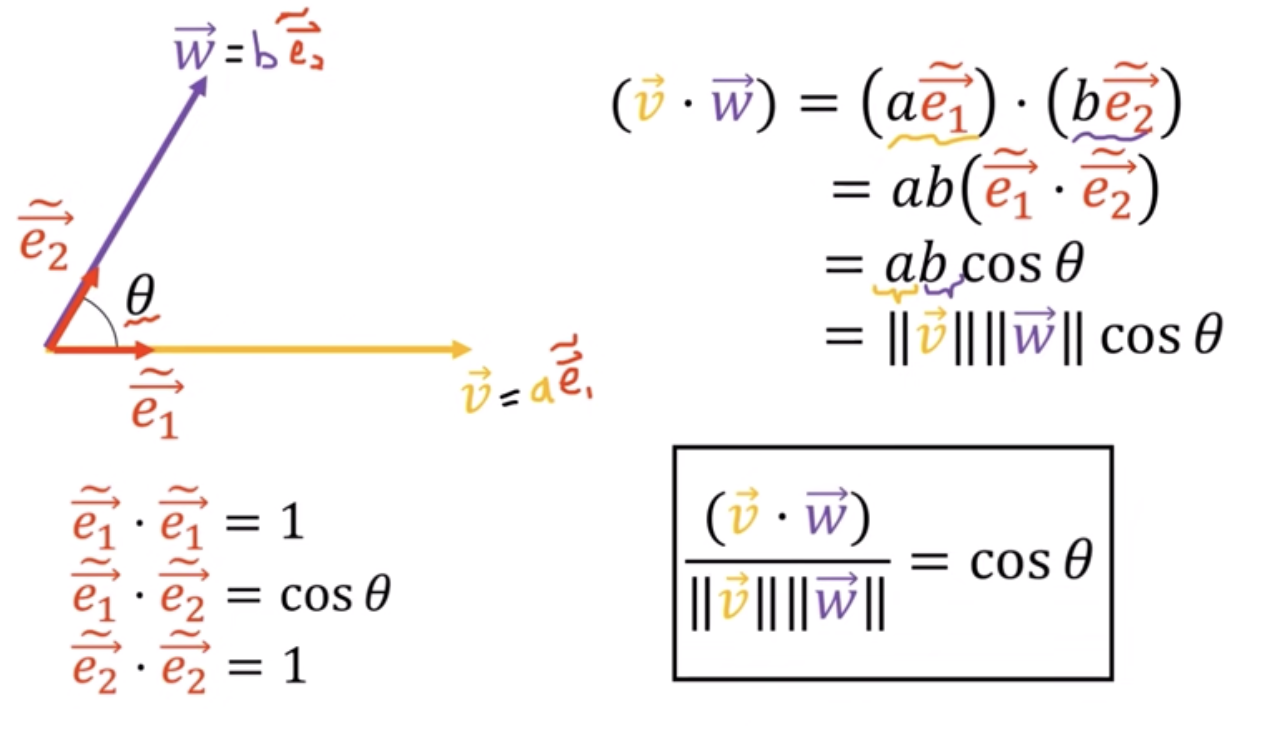
\includegraphics[width=0.6\textwidth]{Angle_between_vectors_dotproduct}
    \caption{Angle $\theta$ between two arbitrary vectors.}
    \label{fig:angle_between_arbitrary_vectors}
\end{figure} \\

To check how the metric tensor transforms, we use the formulation of the metric tensor in
the new system and transform it by replacing the tilde-components by expressing them in
the old system via the definitions of the forward transform given by
equation~(\ref{eq:vector_trafo_overview}):

\begin{equation}
    \begin{array}{rcl}
        \textcolor{red}{\tilde{g}_{ij}} & = & \hdbtv{i} \cdot \hdbtv{j} \\
                       & = & (F^{k~}_{~i}\hdbv{k}) \cdot (F^{l~}_{~j}\hdbv{l}) \\
                       & = & F^{k~}_{~i}  F^{l~}_{~j} (\hdbv{k} \cdot \hdbv{l}) \\
                       \noalign{\vskip10pt}
        \Rightarrow\textcolor{red}{\tilde{g}_{ij}} & = &
        F^{k~}_{~i}  F^{l~}_{~j} \textcolor{MidnightBlue}{{g}_{kl}} \\
        \noalign{\vskip10pt}
        \textcolor{MidnightBlue}{g_{kl}} & = & \hdbv{k} \cdot \hdbv{l} \\
        & = & (B^{i~}_{~k}\hdbtv{i}) \cdot (B^{j~}_{~l}\hdbtv{j}) \\
        & = & B^{i~}_{~k} B^{j~}_{~l} (\hdbtv{i} \cdot \hdbtv{j}) \\
        \noalign{\vskip10pt}
        \Rightarrow \textcolor{MidnightBlue}{g_{kl}} & = &
        B^{i~}_{~k} B^{j~}_{~l} \textcolor{red}{\tilde{g}_{ij}}
    \end{array}
\end{equation} \\

\textcolor{red}{Metric tensors are (0,2)-tensors}. They transform with covariant
transformation behaviour using two consecutive transformations for a change of
coordinates. \\

The metric tensor is a function that takes two vectors as input and transforms them into a
real number, thus it is an example of a so-called bilinear form: $g\!: V \times V
\rightarrow \mathbb{R}$, i.e. $g(\vec{v},\vec{w}) \rightarrow v^i w^j g_{ij}$. When we put
in the same vector twice we get the vector length. When we put in two vectors we get the
product of their vector lengths times the cosine of the angle between them (see
eq.~(\ref{eq:scalar_product_definition})). \\

The metric tensor $g$ is called a bilinear form, because it takes two vectors as input,
maps them to a real number as output, and has the linearity properties for both of its
arguments:
\begin{equation}
    \label{eq:metric_tensor_linearity_properties}
    \begin{array}{rcl}
        g\!: V \times V \rightarrow \mathbb{R},&&
        g(\vec{v},\vec{w}) \rightarrow v^i w^j g_{ij} \\
        \noalign{\vskip10pt}
        a(v^i w^j g_{ij}) &=& (av^i) w^j g_{ij} = v^i (aw^j) g_{ij} \\
        \Rightarrow ag(\vec{v},\vec{w}) &=& g(a\vec{v},\vec{w}) = g(\vec{v},a\vec{w}) \\
        \noalign{\vskip10pt}
        (v^i + u^i) w^j g_{ij} &=& v^i w^j g_{ij} + u^i w^j g_{ij} \\
        \Rightarrow g(\vec{v}+\vec{u},\vec{w}) &=& g(\vec{v},\vec{w}) + g(\vec{u},\vec{w}) \\
        \noalign{\vskip10pt}
        v^i (w^j + t^j) g_{ij} &=& v^i w^j g_{ij} + v^i t^j g_{ij} \\
        \Rightarrow g(\vec{v},\vec{w}+\vec{t}) &=& g(\vec{v},\vec{w}) + g(\vec{v},\vec{t})
    \end{array}
\end{equation}

In general forms are functions that take an arbitrary number of vector inputs and provide
a scalar as an output, i.e. forms: $V \times V \times \cdots \times V \rightarrow
\mathbb{R}$. Forms must have the linearity properties. Examples of a 1-form or a linear form
are covectors ($V \rightarrow \mathbb{R}$). An example of a 2-form or bilinear form is the
metric tensor, as shown above ($V \times V \rightarrow \mathbb{R}$). \\

The metric tensor is a special bilinear form, because it has two additional properties
that bilinear forms do not have in general:
\begin{equation}
    \label{eq:metric_tensor_special_additional_properties}
    \begin{array}{rcl}
        g(\vec{v},\vec{w}) &=& v^i w^j g_{ij} = v^i w^j g_{ji} = g(\vec{w},\vec{v})
        \quad\text{(symmetry)}\\
        g(\vec{v},\vec{v}) &=& \| v \|^2 \geq 0
        \quad\text{(positive vector length)}
    \end{array}
\end{equation} \\

Bilinear forms (including the metric tensor) can alternatively be interpreted as linear
combinations of covector-covector pairs $\mathcal{B} = \mathcal{B}_{ij}
\hdcbvc{i}\hdcbvc{j} = \mathcal{B}_{ij} (\hdcbvc{i} \otimes\hdcbvc{j})$. As for linear
maps, we can show that the bilinear map can be created from that definition and linearity:
\begin{equation}
    \begin{array}{rcl}
        \mathcal{B} & = & \mathcal{B}_{kl} \hdcbvc{k}\hdcbvc{l} \\
        & = & \mathcal{B}_{kl}(F^{k~}_{~i}\hdcbtvc{i})(F^{l~}_{~j}\hdcbtvc{j}) \\
        & = & (F^{k~}_{~i}  F^{l~}_{~j} \mathcal{B}_{kl})\hdcbtvc{i}\hdcbtvc{j} \\
        & = & \widetilde{\mathcal{B}_{ij}}\hdcbtvc{i}\hdcbtvc{j} \\
        \noalign{\vskip10pt}
        \Rightarrow \widetilde{\mathcal{B}_{ij}} & = & F^{k~}_{~i}  F^{l~}_{~j} \mathcal{B}_{kl} \\
        \text{and correspondingly:} \qquad\mathcal{B}_{ij}
        & = & B^{k~}_{~i}  B^{l~}_{~j} \widetilde{\mathcal{B}_{kl}}
    \end{array}
\end{equation}
Their coordinate forms can be derived from this definition $\mathcal{B} = \mathcal{B}_{ij}
\hdcbvc{i}\hdcbvc{j}$ and the vector definitions $\vec{v} = v^k \hdbv{k}$ and $\vec{w} =
w^l \hdbv{l}$ by inserting them:
\begin{equation}
    \begin{array}{rcl}
        s & = & \mathcal{B}(\vec{v},\vec{w}) \\
        & = & \mathcal{B}_{ij}\hdcbvc{i}\hdcbvc{j}(v^k \hdbv{k},w^l \hdbv{l}) \\
        & = & \mathcal{B}_{ij}\hdcbvc{i}(v^k \hdbv{k})\hdcbvc{j}(w^l \hdbv{l}) \\
        & = & \mathcal{B}_{ij}v^k w^l \hdcbvc{i}(\hdbv{k})\hdcbvc{j}(\hdbv{l}) \\
        & = & \mathcal{B}_{ij}v^k w^l \delta^i_k \delta^j_l \\
        & = & \mathcal{B}_{ij}v^i w^j 
    \end{array}
\end{equation} \\

The metric tensor can also be used to describe a correspondence of vectors in the vector
space $V$ to the dual space $V^*$. The correspondence exists between vectors and the
scalar product of $\vec{v}$ with an open slot to be filled with another vector. This leads
to a formula for lowering the index of a vector component with the help of the metric
tensor $g_{ij}$ and a formular for raising the index with the help of the inverse metric
tensor $\mathfrak{g}^{ij}$:
\begin{equation}
    \begin{array}{rclrcl}
        v_i & = & g_{ij} v^j \qquad 
        \widetilde{v_i} & = & \widetilde{g_{ij}} \widetilde{v^j} \\
        v^i & = & \mathfrak{g}^{ij} v_j \qquad 
        \widetilde{v^i} & = & \widetilde{\mathfrak{g}^{ij}} \widetilde{v_j} \\
        \text{where}\quad \mathfrak{g}^{ki}g_{ij} & = &  \delta^k_j \qquad
        \widetilde{\mathfrak{g}^{ki}}\widetilde{g_{ij}} & = & \delta^k_j
    \end{array}
\end{equation} \\

\newpage